\begin{boxC}
    الگوریتم
    \lr{PageRank}
    در واقع به صورت زیر عمل می‌کند که وزن (رتبه) عددی را به هر گره در نمودار اختصاص می دهد که نشان دهنده اهمیت یا اعتبار آن است.

رتبه را بر اساس تعداد و کیفیت لینک های ورودی به یک گره محاسبه می کند.

مرتباً رتبه ها را تا رسیدن به همگرایی به روز می کند.

اما رویکرد الگوریتم 
\lr{Hub}
به این صورت است که 
دو نوع گره را شناسایی می کند: مقامات (منابع محتوای با کیفیت بالا) و هاب (صفحاتی که به بسیاری از مقامات پیوند دارند).
امتیازات اعتبار را بر اساس تعداد و کیفیت لینک های دریافتی از هاب محاسبه می کند.
امتیازات هاب را بر اساس تعداد و کیفیت پیوندهای خروجی به مقامات محاسبه می کند.
به طور مکرر امتیازها را تا رسیدن به همگرایی به روز می کند.

% 1000 گره اصلی مشترک بین رتبه صفحه و امتیازات 
۱۰۰۰ گره مشترک بین این دو الگوریتم 
 صفحاتی را نشان می دهد که هم بسیار معتبر هستند و هم
  به خوبی متصل است
این صفحات احتمالاً مرتبط هستند، زیرا هم توسط منابع معتبر دیگر و هم صفحاتی که به بسیاری از منابع معتبر پیوند دارند تأیید شده اند.


\lr{PageRank}
همه پیوندهای ورودی را به طور مساوی درنظر می‌گیرد ، در حالی که 
\lr{HITS}
بین پیوندها از هاب و غیرهاب تمایز قائل می‌شود.

الگوریتم
\lr{PageRank}
با در نظرگرفتن کل ساختار به صورت
\lr{global}
تر عمل می‌کند در حالی که 
\lr{HITS}
محلی‌تر عمل می‌کند و بر همسایگی گره تمرکز دارد.

\end{boxC}

\begin{boxC}
    اندازه تعداد رئوس بزرگترین مولفه همبندی ضعیف این گراف : 855802

    اندازه تعداد یال‌های رئوس بزرگترین مولفه همبندی ضعیف این گراف : 5066841
\end{boxC}

\begin{figure}
    \centering
    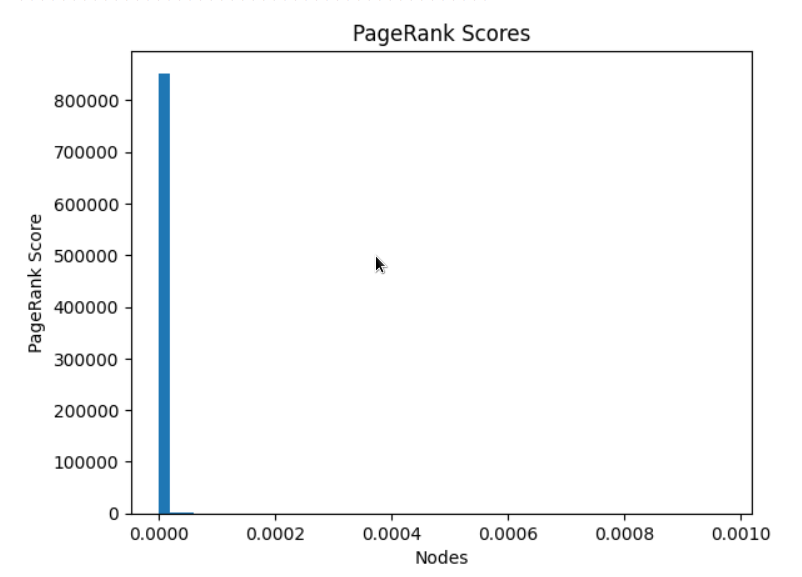
\includegraphics
    [width = 0.65\textwidth]
    {IR5/image/PageRankScores.png}
    \caption{\lr{PageRank Scores Histogram}}
    \label{fig:enter-label}
\end{figure}


\begin{figure}
    \centering
    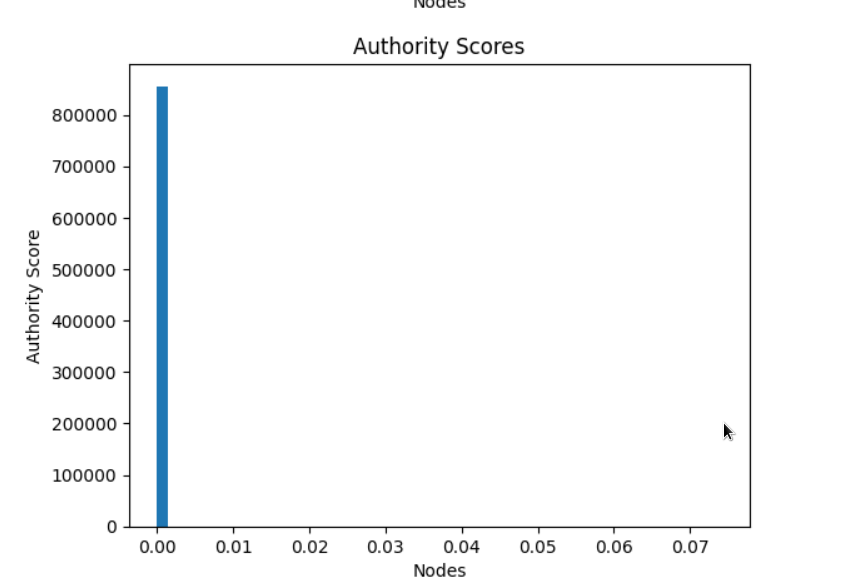
\includegraphics
    [width = 0.65\textwidth]
    {IR5/image/AuthorityScores.png}
    \caption{\lr{Authority Scores Histogram}}
    \label{fig:enter-label}
\end{figure}

\begin{figure}
    \centering
    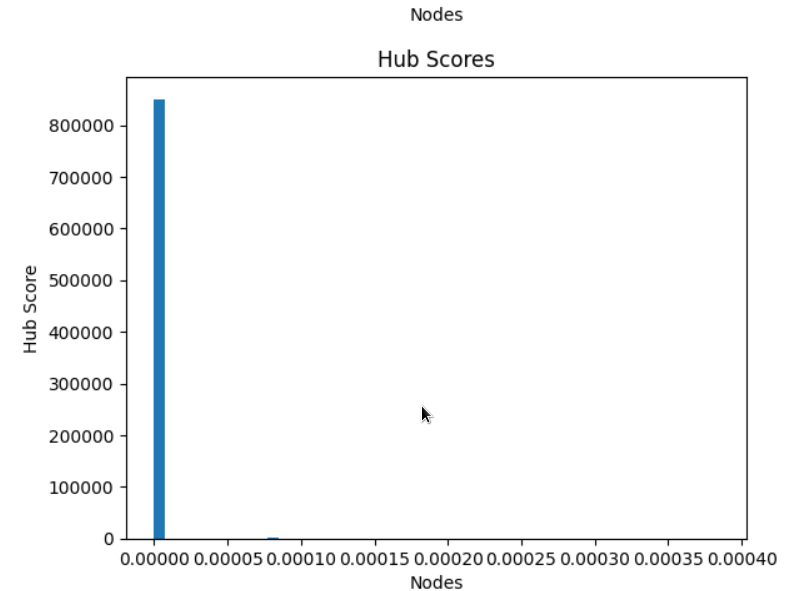
\includegraphics
    [width = 0.65\textwidth]
    {IR5/image/HubScores.png}
    \caption{\lr{Hub Scores Histogram}}
    \label{fig:enter-label}
\end{figure}

\begin{figure}
    \centering
    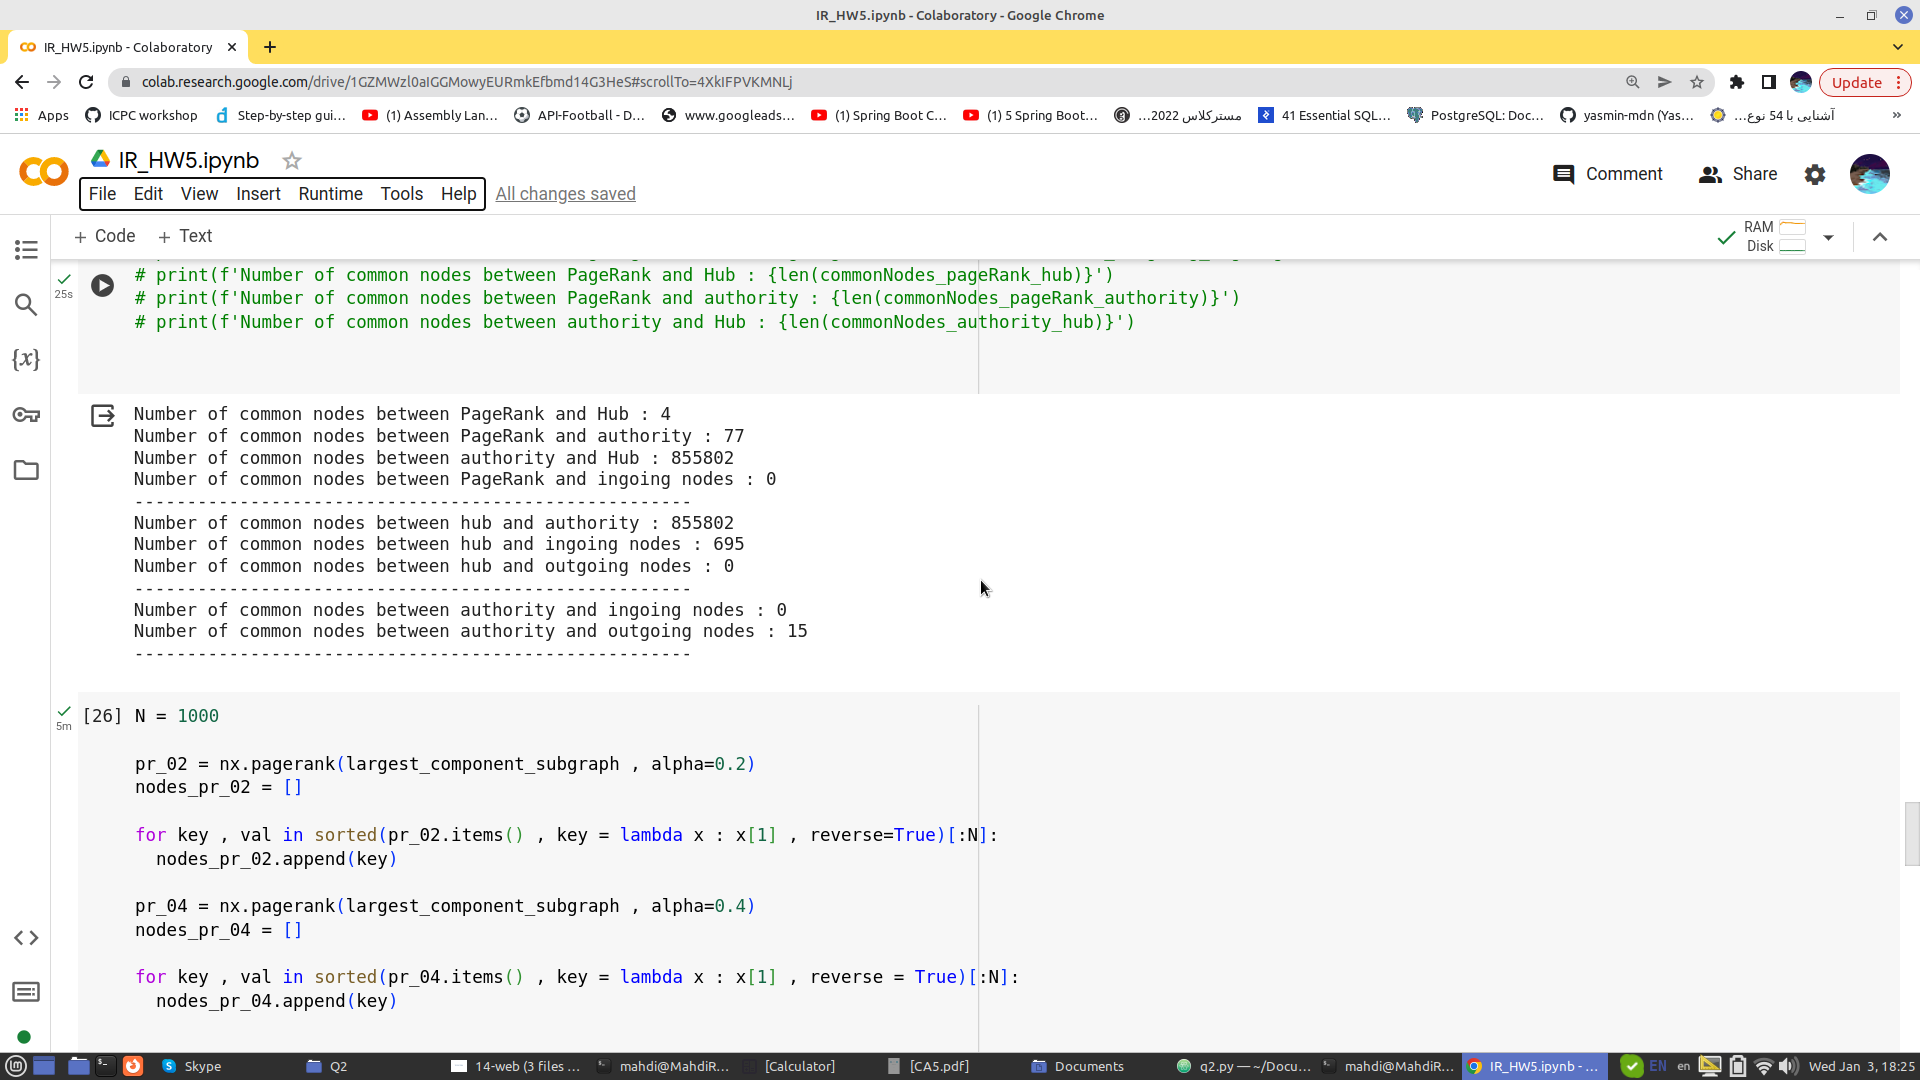
\includegraphics
    [width = 0.8\textwidth]
    {IR5/image/PR_2.png}
    \caption{میزان اشتراک در بین نقاط در میان رویکردهای امتیازدهی}
    \label{fig:enter-label}
\end{figure}

\begin{figure}
    \centering
    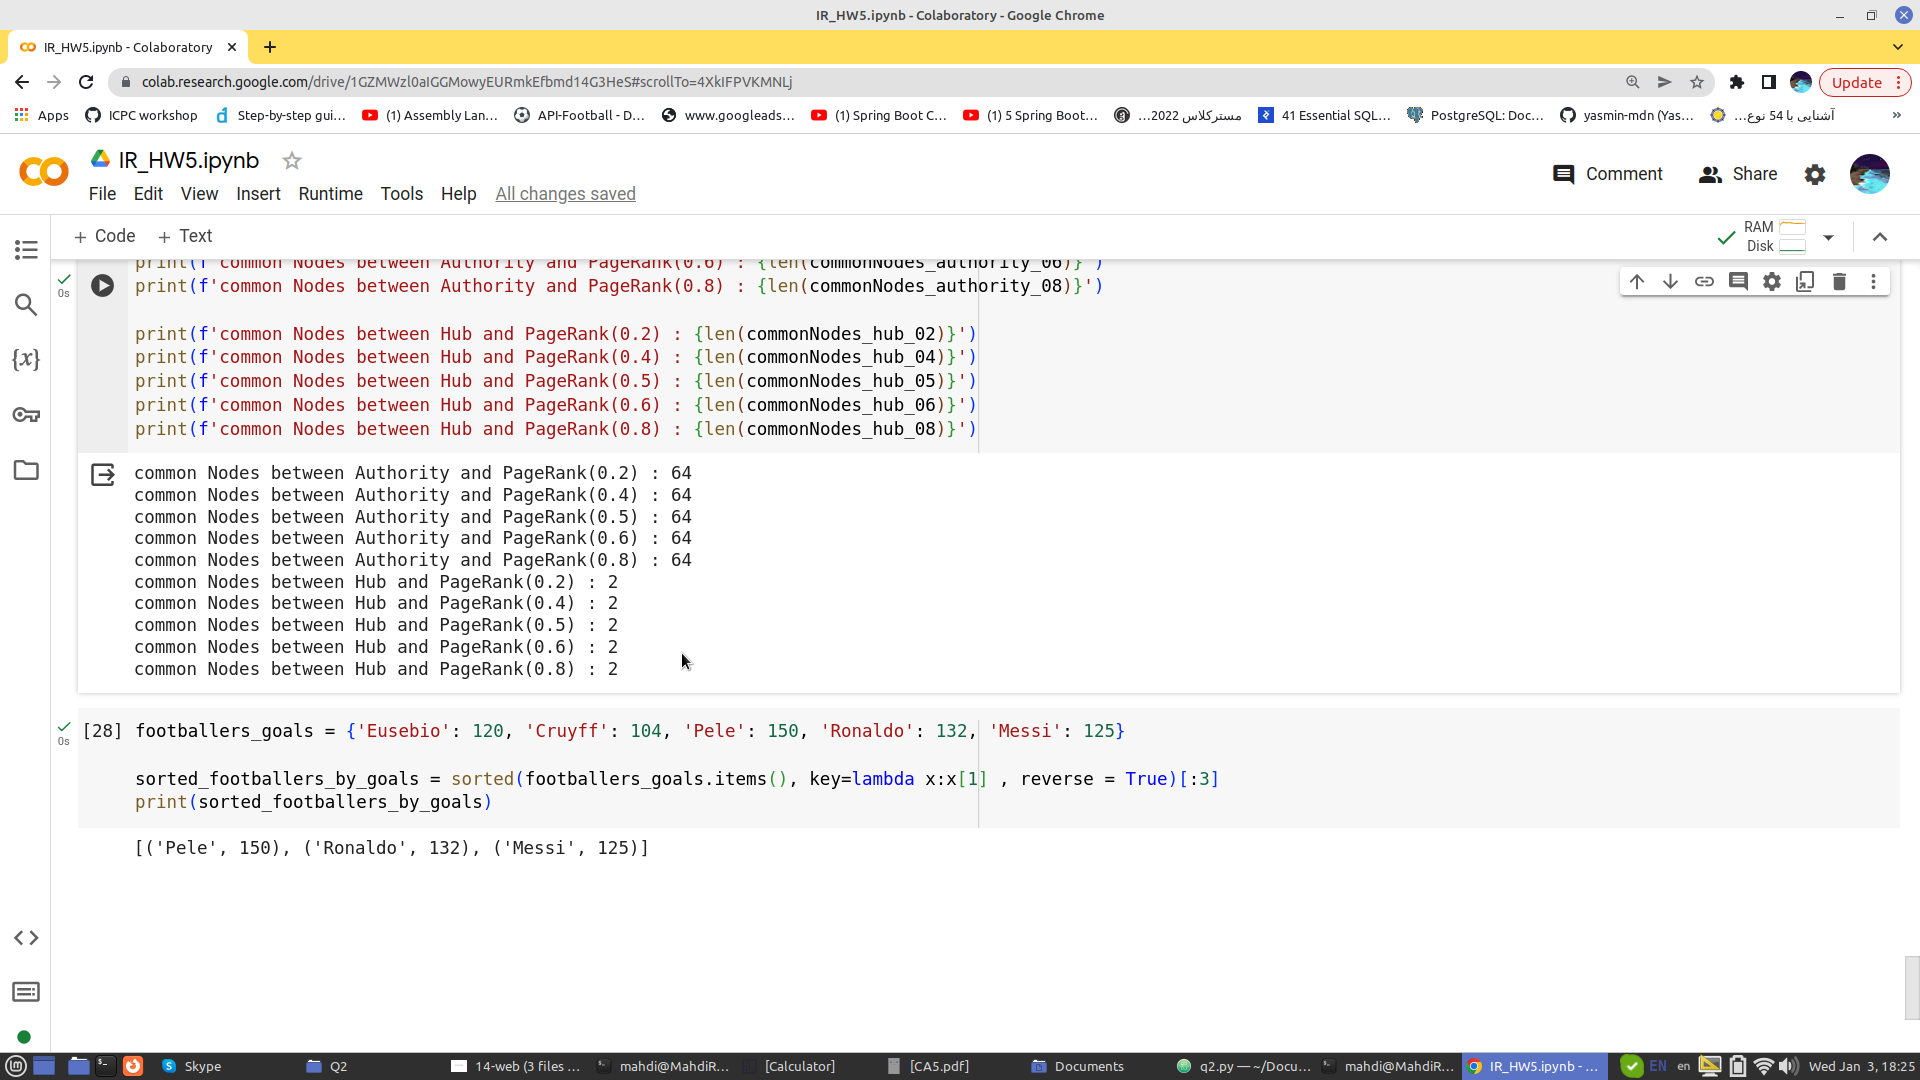
\includegraphics
    [width = 0.8\textwidth]
    {IR5/image/PR_3.png}
    \caption{میزان اشتراک در بین نقاط در میان رویکردهای امتیازدهی}
    \label{fig:enter-label}
\end{figure}